\chapter{The Sensory Afferent Database}\label{ch:database}
\graphicspath{{figs/50-database/}}

\section{The Resource}\label{sec:sadb_resource}

The Sensory Afferent Database (SADb) is a curated literature resource for studying sensory feedback in locomotion and posture. It connects papers to afferent classes, experimental preparations, feedback pathways, and computational models. I developed it within the AARL's NeuroNex Communication, Coordination, and Control in Nervous Systems (C3NS) effort and presented the resource at Neuroscience 2023 \citep{bolen_sensory_2023}.

The knowledge gap was the lack of a structured account, available to this project, of which measured afferent properties and feedback pathways could support the robot's controller. Relevant findings were dispersed across species, preparations, tasks, and primary papers. Reviews organized parts of this evidence \citep{van_de_crommert_review_1998, windhorst_muscle_2007, windhorst_spinal_2022}, but selecting a feedback rule still required recovering its experimental conditions and separating measurements from modeling assumptions. I built SADb to connect those findings to their sources, afferent classes, and pathway roles so that controller choices could be traced to the evidence and remaining unknowns could be identified.

The primary deliverable is a browser application for searching paper records, counting them by selected classifications, and exploring citation neighborhoods (Figure~\ref{fig:sadb_clusters}). Its embedded data support offline use; its separate online-search tab requires a network connection. The distributed snapshot contains 1,393 records: 943 papers and 450 linked model, review, feedback-pathway, and recorder records. Archived records remain available alongside the retained collection. The pivot and citation views operate on papers; the table view searches across record types.

The working base in Airtable contains linked Papers, Feedback, Models, Review Papers, and Recorders tables. Papers hold bibliographic information and curation notes: short summaries of the reported mechanism, experimental conditions, and relevance to feedback design, grounded in the source text. Feedback records describe a sensory pathway, such as Ib feedback influencing the stance-to-swing transition, and link it to supporting papers; Models link computational implementations to their source literature. The other tables organize review literature and recording methods. Paper matching uses DOI where available and normalized titles otherwise. The paper-table view is shown in Appendix~\ref{app:sadb_records} (Figure~\ref{fig:sadb_explorer}). I curate the linked Airtable base and rebuild the read-only application from its exported records.

\begin{figure}[htbp]
\centering
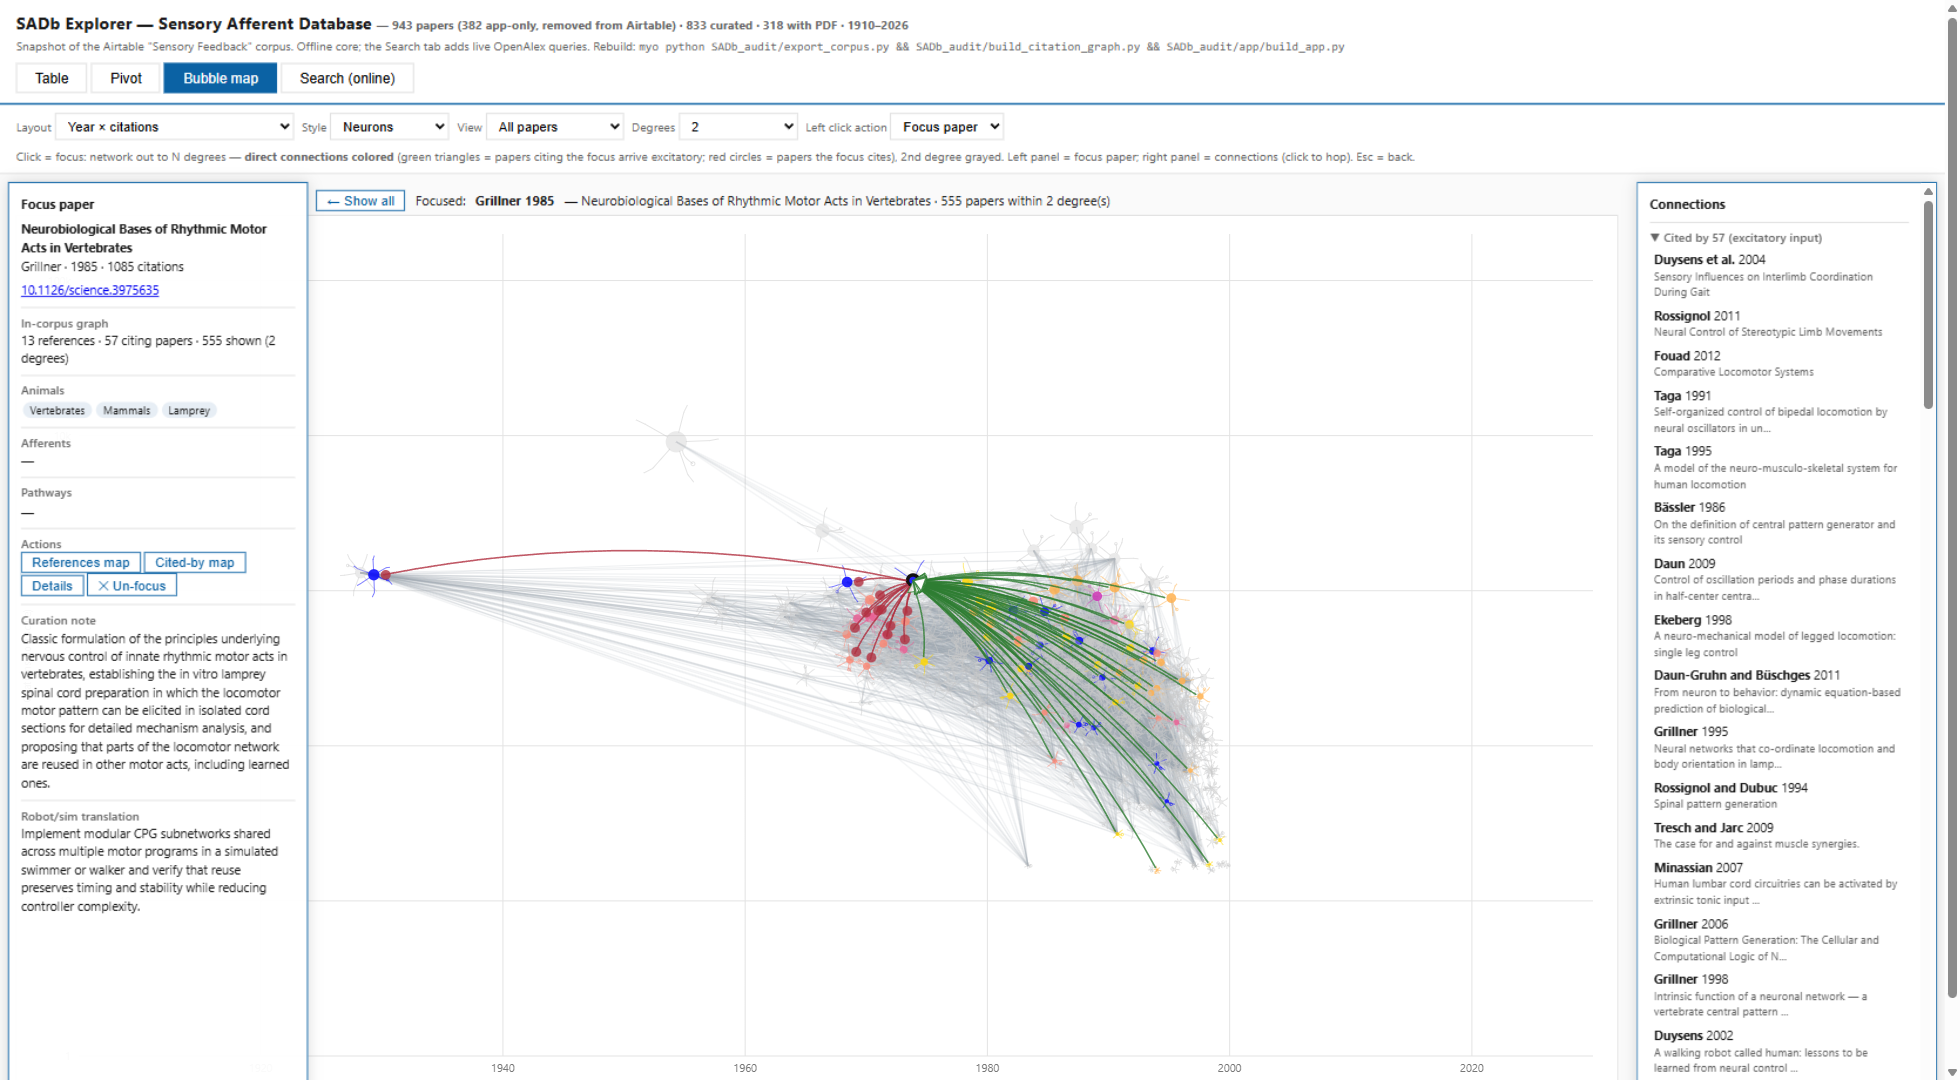
\includegraphics[width=0.94\textwidth]{sadb_clusters_app.png}
\caption[SADb citation-neighborhood view]{Paper-only citation view focused on Grillner (1985). Soma size represents citation count; axes show year and citation count. Triangles mark 57 in-corpus citers, and circles 13 cited papers. Second-degree papers are gray. The panels identify the selected paper and its connections.}
\label{fig:sadb_clusters}
\end{figure}

\section{Curation Methods}\label{sec:sadb_methods}

The collection began with my Zotero library, the laboratory's Biology library, and the papers already curated in Airtable. Records were reconciled by DOI and title, then expanded through citation searches and the laboratory's PDF collection. Reviews of spinal and proprioceptive feedback supplied an initial organization of the literature \citep{van_de_crommert_review_1998, windhorst_muscle_2007, windhorst_spinal_2022}. This was a curated research collection, rather than a registered systematic review or an exhaustive search of every relevant publication.

Records were retained when they reported sensory-afferent measurements, investigated feedback in locomotion or posture, or modeled a relevant sensory pathway. Reviews were retained as sources for organizing and locating that evidence. Duplicate records and material outside this feedback scope were removed from the working base. Classification used controlled vocabularies for preparations and afferent classes. Each mechanism summary was grounded in available source text, using the abstract when full text was unavailable; missing text was flagged rather than supplied from recollection. The retained and archived sets distinguish the working collection from the broader audit.

\subsection{AI-Assisted Triage}\label{sec:sadb_triage}

I evaluated AI-assisted literature triage in work presented at Neuroscience 2024 \citep{bolen_using_2024}. AI tools helped draft and classify records, but their output required checking against the source. I retained responsibility for inclusion, classification, and deletion decisions. The role of these tools was to assist curation, not to establish the correctness of a physiological claim. Their use does not make the corpus complete or remove the need to inspect the underlying papers.

\section{Coverage and Use}\label{sec:sadb_corpus}

The audited paper set contains 943 records; 561 were retained in the working base. Of those retained papers, 523 have curation notes, 426 have preparation tags, 86 have an afferent classification, and 258 have notes relating their findings to robot or simulation use. These counts describe curation coverage, not the number of independent physiological findings or a measure of their reliability. The more detailed record counts and linked pathway examples are given in Appendix~\ref{app:sadb_records}.

A user can begin with a preparation or afferent class, retrieve the matching papers, and inspect their notes and source links. The pivot view counts papers along two selected dimensions (Figure~\ref{fig:sadb_pivot}); the citation view provides a second route from an anchor paper to related literature (Figure~\ref{fig:sadb_clusters}). These views help locate evidence, while the original experiment determines the conditions under which a finding applies.

\begin{figure}[htbp]
\centering
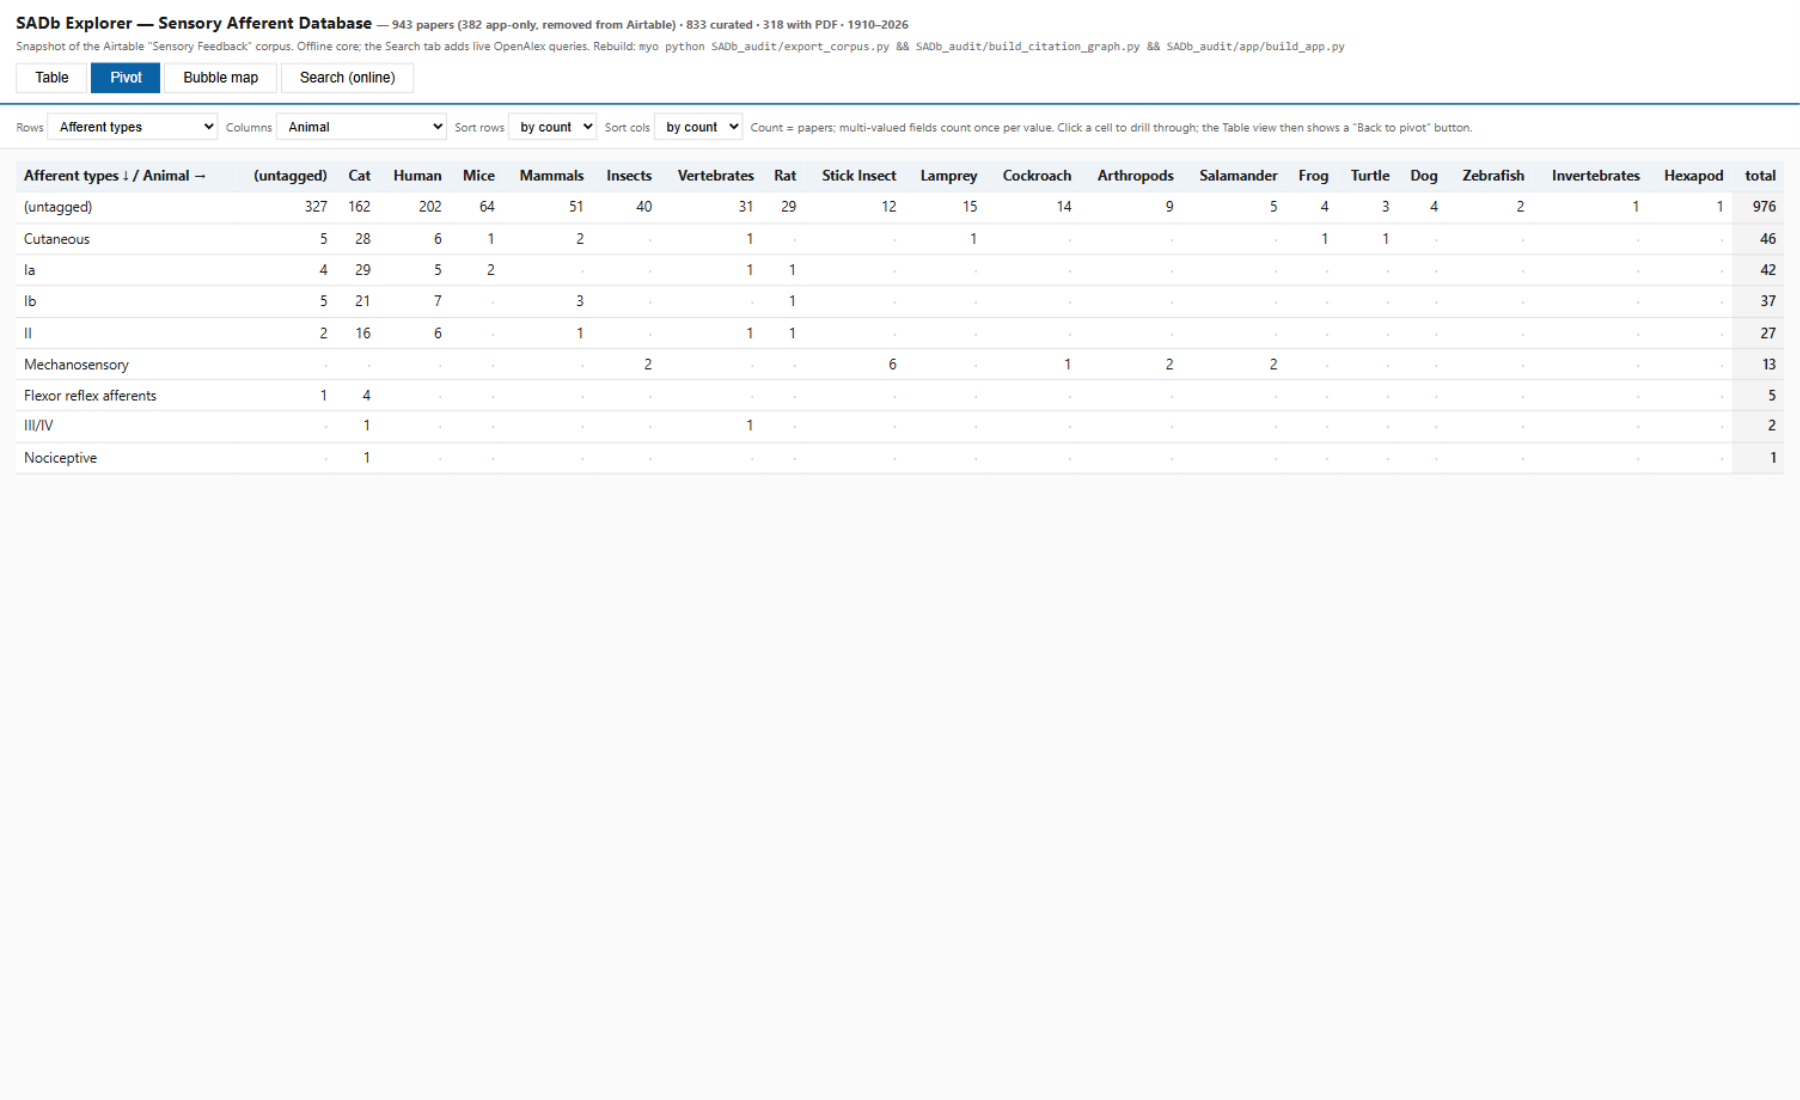
\includegraphics[width=0.96\textwidth,trim=0 610bp 980bp 150bp,clip]{sadb_pivot_app.png}
\caption[The SADb Explorer pivot view]{Excerpt of the application pivot matrix, with afferent classifications as rows and selected animal preparations as columns. Cells count tagged papers; selecting a cell retrieves its records. Multiple tags allow a paper to contribute to more than one cell.}
\label{fig:sadb_pivot}
\end{figure}

\subsection{Use in Neural-Controller Design}\label{sec:sadb_use}

The resource helped organize the sensory channels used in Chapter~\ref{ch:sns}: spindle-related length and velocity signals, force feedback, and contact events. The linked records provide sources for selecting a pathway and examining its preparation, sign, and phase dependence. They are not ready-made controller parameters. Translating an experimental result into a robot circuit still requires decisions about sensor encoding, species and task differences, and gain selection, followed by verification of the implemented behavior.

The present corpus is uneven. Its afferent classifications cover only part of the retained literature, and the depth of the mammalian locomotor material should not be taken as equal coverage of vestibular, visual, or other sensory systems. The application makes the curated papers easier to inspect and compare; additional curation and experimental interpretation remain necessary for extending the robot's sensory system.
